\documentclass[a4paper,fleqn]{cas-dc}

% If the frontmatter runs over more than one page
% use the longmktitle option.

%\documentclass[a4paper,fleqn,longmktitle]{cas-dc}

%\usepackage[numbers]{natbib}
%\usepackage[authoryear]{natbib}
\usepackage[authoryear,longnamesfirst]{natbib}

%%%Author macros
% \def\tsc#1{\csdef{#1}{\textsc{\lowercase{#1}}\xspace}}
% \tsc{WGM}
% \tsc{QE}
%%%

% Uncomment and use as if needed
%\newtheorem{theorem}{Theorem}
%\newtheorem{lemma}[theorem]{Lemma}
%\newdefinition{rmk}{Remark}
%\newproof{pf}{Proof}
%\newproof{pot}{Proof of Theorem \ref{thm}}

\begin{document}
\let\WriteBookmarks\relax
\def\floatpagepagefraction{1}
\def\textpagefraction{.001}

% Short title
% \shorttitle{<short title of the paper for running head>}    

% Short author
% \shortauthors{<short author list for running head>}  

% Main title of the paper
\title [mode = title]{HCAUV:A Tri-Cabin AUV with Numerical Models and Robust Control Scheme to Improve Maneuverable Capabilities}  

% Title footnote mark
% eg: \tnotemark[1]
% \tnotemark[1] 

% Title footnote 1.
% eg: \tnotetext[1]{Title footnote text}
% \tnotetext[1]{Title footnote text} 

% First author
%
% Options: Use if required
% eg: \author[1,3]{Author Name}[type=editor,
%       style=chinese,
%       auid=000,
%       bioid=1,
%       prefix=Sir,
%       orcid=0000-0000-0000-0000,
%       facebook=<facebook id>,
%       twitter=<twitter id>,
%       linkedin=<linkedin id>,
%       gplus=<gplus id>]

\author[1]{Rui Yang}[type=editor,
        style=chinese,
        auid=1,bioid=1]
% Corresponding author indication
\cormark[1]
\fnmark[1] 

% Footnote of the first author
\ead{yangrui@ouc.edu.cn}
% Email id of the first author

% URL of the first author
% \ead[url]{<URL>}

% Credit authorship
% eg: \credit{Conceptualization of this study, Methodology, Software}
% \credit{<Credit authorship details>}

% Address/affiliation
\affiliation[1]{organization={Ocean University of China},
            % addressline={13}, 
            city={Qingdao},
%          citysep={}, % Uncomment if no comma needed between city and postcode
            postcode={266100}, 
            % state={},
            country={China}}

\author[1]{Xuchen Feng}[style=chinese]

% Footnote of the second author
\ead{fxc@stu.ouc.edu.cn}

% Email id of the second author
% \ead{}

% URL of the second author
% \ead[url]{}

% Credit authorship
% \credit{}

% Address/affiliation
% \affiliation[2]{organization={Ocean University of China},
%             % addressline={}, 
%             city={Qingdao},
% %          citysep={}, % Uncomment if no comma needed between city and postcode
%             postcode={266100}, 
%             % state={},
%             country={China}}

% Corresponding author text
\cortext[1]{Corresponding author}

% Footnote text
% \fntext[1]{}

% For a title note without a number/mark
%\nonumnote{}

% Here goes the abstract
\begin{abstract}[S U M M A R Y]
  This is the abstract. This is the abstract. This is the abstract. This is the abstract. 
  This is the abstract. This is the abstract. This is the abstract. This is the abstract. 
  This is the abstract. This is the abstract. This is the abstract. This is the abstract. 
  This is the abstract. This is the abstract. This is the abstract. This is the abstract. 
  This is the abstract. 
\end{abstract}

% Use if graphical abstract is present
%\begin{graphicalabstract}
%\includegraphics{}
%\end{graphicalabstract}

% Research highlights
% \begin{highlights}
% \item highlights1

% \item highlights2

% \item highlights3
% \end{highlights}

% Keywords
% Each keyword is seperated by \sep
\begin{keywords}
  AUV design \sep Hydrodynamic Modling \sep \emph{$H_\infty$} Robust Control \sep 
\end{keywords}

\maketitle

% Main text
\section{Inroduction}\label{Indro}
This is the Introduction.This is the Introduction.This is the Introduction.This is the Introduction.
This is the Introduction.This is the Introduction.This is the Introduction.This is the Introduction.
This is the Introduction.This is the Introduction.This is the Introduction.This is the Introduction. 

\begin{figure}
	\centering
		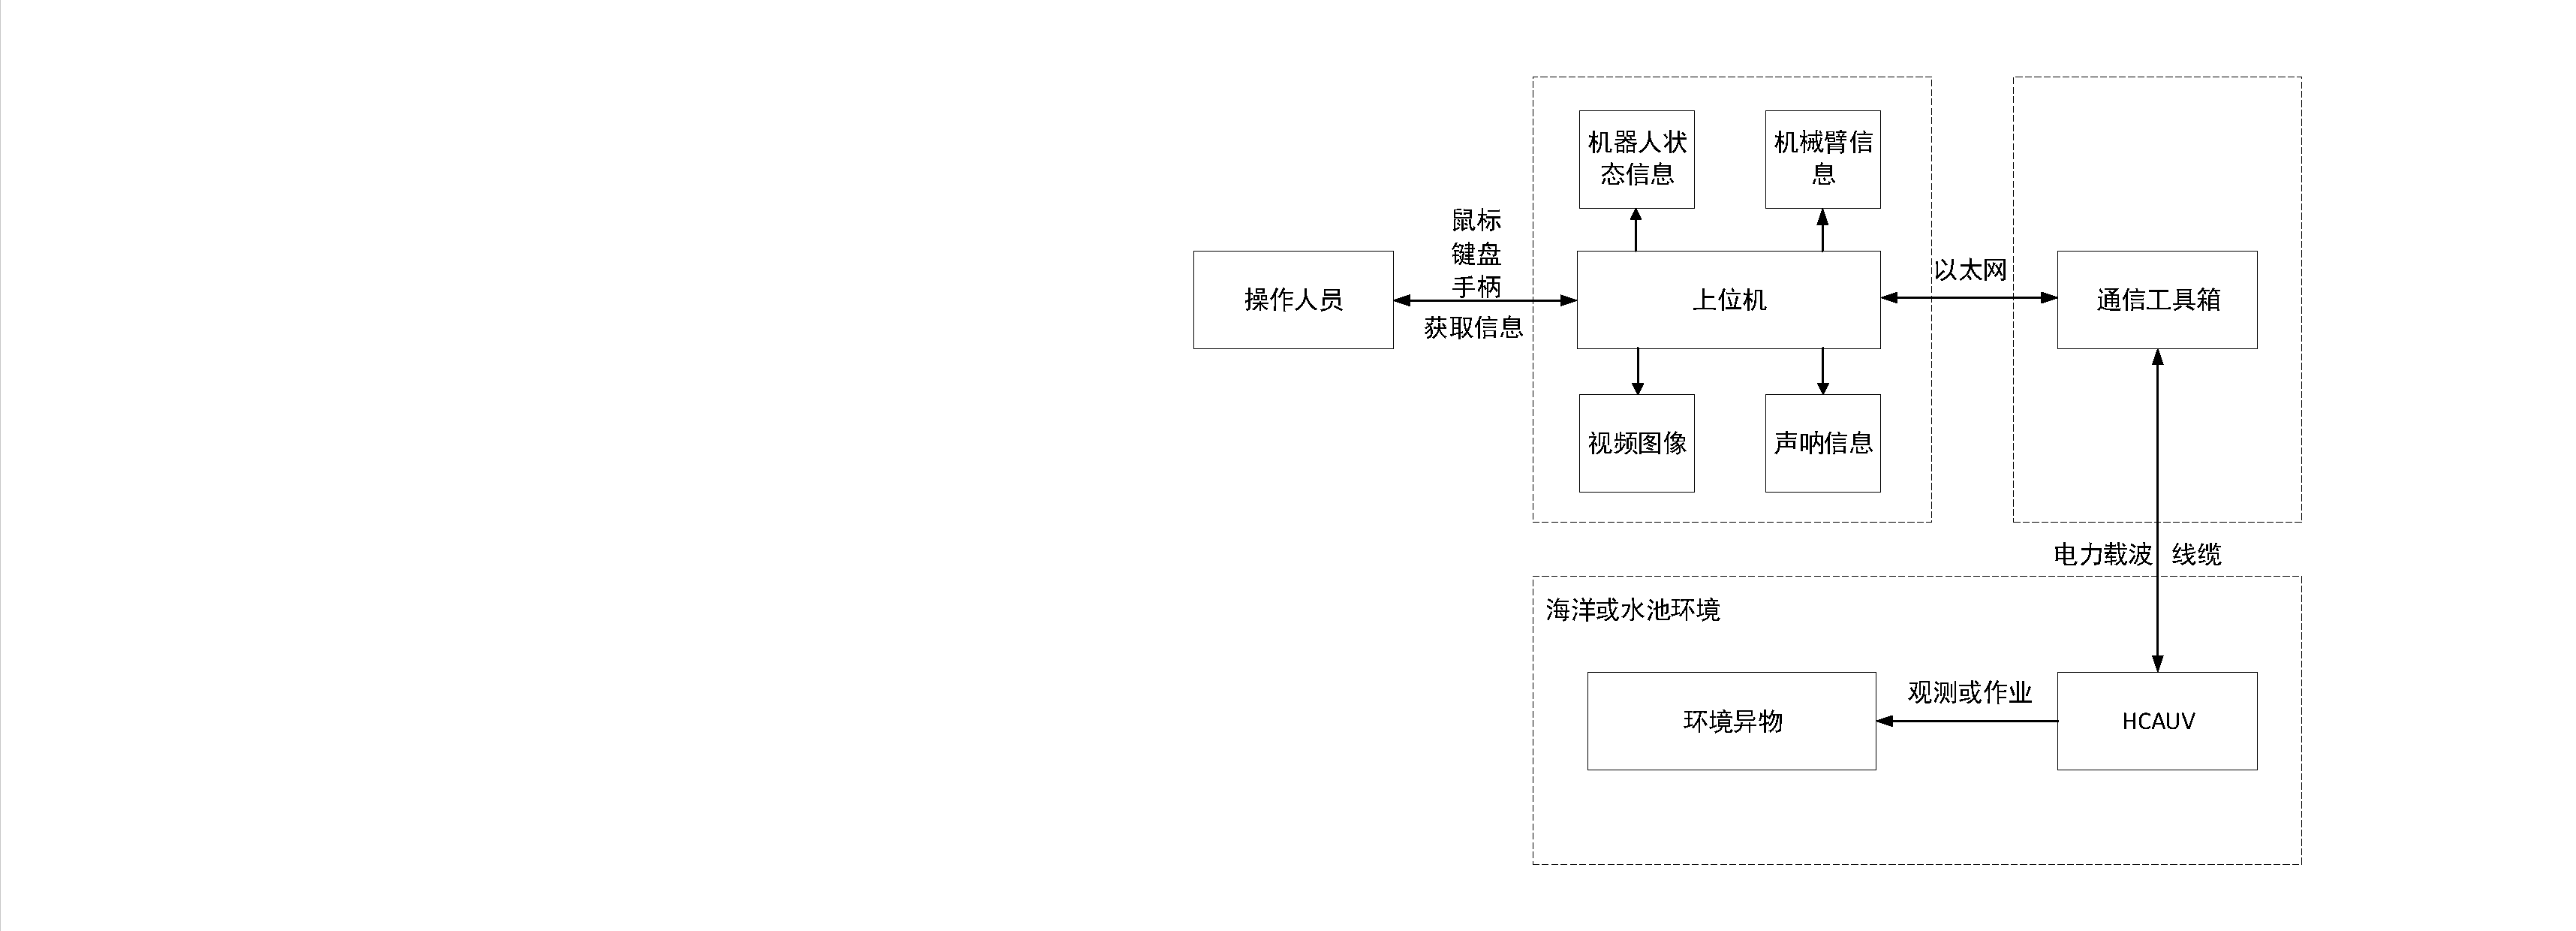
\includegraphics[width=5cm,height=3cm]{1}
	  \caption{123546546}
    \label{fig1}
\end{figure}

\section{Development of HCAUV}
This is Development of HCAUV. This is Development of HCAUV. This is Development of HCAUV. This is Development of HCAUV.
This is Development of HCAUV. This is Development of HCAUV. This is Development of HCAUV. This is Development of HCAUV. 
This is Development of HCAUV. This is Development of HCAUV.  

\subsection{Structural design}
This is Structural design. This is Structural design. This is Structural design. 

\subsection{Buoyancy shell design}
This is Buoyancy shell design. This is Buoyancy shell design. This is Buoyancy shell design. 

\subsection{Thruster configuration}
This is Thruster configuration. This is Thruster configuration.This is Thruster configuration.


\section{Hydrodynamic Modeling}
This is Hydrodynamic Modeling.

\section{\emph{$H_\infty$} Robust Control}
This is Robust Control.

\section{Experimental result}
This is Experimental result.

\section{Conclusion}
This is Conclusion. This is Conclusion.This is Conclusion.This is Conclusion.This is Conclusion.
This is Conclusion.This is Conclusion.This is Conclusion.This is Conclusion.This is Conclusion.
This is Conclusion.This is Conclusion.This is Conclusion.This is Conclusion.
% Numbered list
% Use the style of numbering in square brackets.
% If nothing is used, default style will be taken.
%\begin{enumerate}[a)]
%\item 
%\item 
%\item 
%\end{enumerate}  

% Unnumbered list
%\begin{itemize}
%\item 
%\item 
%\item 
%\end{itemize}  

% Description list
%\begin{description}
%\item[]
%\item[] 
%\item[] 
%\end{description}  

% Figure
% \begin{figure}[<options>]
% 	\centering
% 		\includegraphics[<options>]{}
% 	  \caption{}\label{fig1}
% \end{figure}


% \begin{table}[<options>]
% \caption{}\label{tbl1}
% \begin{tabular*}{\tblwidth}{@{}LL@{}}
% \toprule
%   &  \\ % Table header row
% \midrule
%  & \\
%  & \\
%  & \\
%  & \\
% \bottomrule
% \end{tabular*}
% \end{table}

% Uncomment and use as the case may be
%\begin{theorem} 
%\end{theorem}

% Uncomment and use as the case may be
%\begin{lemma} 
%\end{lemma}

%% The Appendices part is started with the command \appendix;
%% appendix sections are then done as normal sections
%% \appendix

% \section{}\label{}

% To print the credit authorship contribution details
% \printcredits

% %% Loading bibliography style file
% %\bibliographystyle{model1-num-names}
% \bibliographystyle{cas-model2-names}

% % Loading bibliography database
% \bibliography{}

% Biography
% \bio{}
% % Here goes the biography details.
% \endbio

% \bio{pic1}
% % Here goes the biography details.
% \endbio

\end{document}

